% !TEX program = pdflatex
\documentclass[12pt, english]{article}

\usepackage[T1]{fontenc}
\usepackage[utf8]{inputenc}
\usepackage[english]{babel}
\usepackage{ragged2e} 
\usepackage{setspace}
\usepackage[compress]{natbib}
\usepackage{amsmath}
\usepackage{graphicx}
\usepackage{caption, subcaption}
\usepackage{booktabs}
\usepackage{threeparttable}
\usepackage{longtable}
\usepackage{xcolor}
%\usepackage[hypertexnames=false]{hyperref}
\usepackage[hidelinks]{hyperref}
\usepackage{lscape}
\usepackage{ebgaramond}

\usepackage[page,header]{appendix}
\usepackage{lipsum}
\DeclareOption*{\PassOptionsToClass{\CurrentOption}{article}}
\ProcessOptions
\RequirePackage{titletoc}

\usepackage[export]{adjustbox}


\newcommand{\fignote}[2]{\begin{center}\parbox[c]{#1}{\footnotesize #2} \end{center}}
\newcommand{\tabnote}[2]{\begin{center}\parbox[c]{#1}{\footnotesize #2} \end{center}}
\providecommand{\set}[1]{\left\lbrace#1\right\rbrace}

\usepackage{epigraph}

%%%%%%%% Edit at your own risk %%%%%%%%%
\pagestyle{plain}                     %%
%%%%%%%% EXACT 1in MARGINS %%%%%%%%%%%%%
\setlength{\textwidth}{6.5in}     %%  %%
\setlength{\oddsidemargin}{0in}   %%  %%
\setlength{\evensidemargin}{0in}  %%  %%
\setlength{\textheight}{8.75in}   %%  %%
\setlength{\topmargin}{0in}       %%  %%
\setlength{\headheight}{0in}      %%  %%
\setlength{\headsep}{0in}         %%  %%
\setlength{\footskip}{.5in}       %%  %%
%%%%%%%%%%%%%%%%%%%%%%%%%%%%%%%%%%%%%%%%


%\hypersetup{nolinks=true}

\newcommand{\specialcell}[2][r]{%
  \begin{tabular}[#1]{@{}c@{}}#2\end{tabular}}




\title{Can scientific information address vaccine hesitancy? A randomized controlled trial \thanks{We thank seminar audiences 
at the University of Wisconsin-Madison and the Booth Health Economics Summit for helpful comments. Support for this research was 
provided by the National Pharmaceutical Council.
}}
\author{Daniel W. Sacks\thanks{%
  Risk \& Insurance, Wisconsin School of Business, University of Wisconsin - Madison 
  (dan.sacks@wisc.edu).}
 \and
Brigham Walker\thanks{%
  Weatherhead School of Tropical Medicine and Public Health, Tulane University
  (brigham.walker@tulane.edu).} 
}
\date{\today \\ \vspace{0.5em} \large\textbf{Preliminary and incomplete. Please do not cite or circulate.}}

\begin{document}

\begin{spacing}{0.9}
\begin{titlepage}
\maketitle

\thispagestyle{empty}



\begin{abstract}
\input{abstract}
\end{abstract}
\vspace{0.2in}
{{\small JEL codes: D83, I12, I18, L65
\\ 
Key words: vaccines, belief elicitation, demand estimation }}

\end{titlepage}
    
\end{spacing}

\onehalfspacing


\section{Introduction} 
    \label{sec:intro}
    Since the COVID-19 pandemic, vaccination rates have fallen across a wide category of diseases. 
The share of kindergartners not vaccinated against measles, mumps, and urbella increased from 4 
percent in 2020 to 6 percent in 2025; polio and hepatitis-B vaccination rates fell similarly
\citep{cdc_schoolvaxview_data}.
Adult vaccination rates have fallen as well, with flu vaccination rates falling each year 
since 2020 \citep{cdc_flu_vaccinations_weekly}.
These declining vaccination rates are concerning given the health benefits of vaccination 
and widespread scientific evidence supporting the safety and effectiveness of vaccination.

Many interventions have been tested to address declining vaccination rates, but with limited 
success, especially for vaccine hesitant people. 
For example, nudges and reminders can raise flu vaccination rates by 1-3 percentage points 
\citep{milkman2022680,patel2023randomized}, but reminders had mixed effects among the hesitant 
\citep{chang2023reminders,chang2026impact} Incentives raised vaccination rates COVID booster 
rates by A-B percentage points, among people who had already received a primary shot 
\citep{campos2024incentives}. Incentives in the US among vaccine hesitant Americans produced 
much smaller increases \citep{chang2023reminders, chang2026impact}.

The limited success of nudges, reminders, and incentives indicates that Increasing vaccination rates among vaccine hesitant people may require changing their beliefs about the benefits and costs of vaccination, 
although doing so in practice has proven challenging. Addressing beliefs via information provision has yielded mixed results: dispelling myths did not increase flu or pediatric vaccination rates 
\citep{nyhan2014effective, nyhan2015does}, 
while highlighting harms of pediatric illness raised support for pediatric vaccinations \citep{horne2015countering}.
Endorsements from trusted messengers may help \citep{larsen2023counter,alsan2024experimental}, albeit with modest effect sizes.  

In this paper, we test whether providing scientific evidence about flu vaccine side effects to vaccine hesitant people can shift beliefs about their own risks from the flu vaccine. 
Scientific information provides part of the basis for the widespread recommendation to evaluate---establishing the safety of vaccines---so it is natural to communicate. However it may not influence 
beliefs if vaccine hesitant participants do not trust the information source or do not believe it is relevant to them. 

We focus on the flu vaccine because flu remains an important seasonal disease, killing tens of thousands of Americans annually and infecting tens of millions. 
We focus on side effect beliefs because prior work has shown that flu vaccine hesitancy is strongly associated with pessimistic beliefs about sides \citep{chapman1999predictors,tsutsui2012economic}.
Quantitative belief elicitations show that vaccine hesitant people believe the flu vaccine side effect rate is 7-15 percentage points on average, 
much higher than clinical trial reports \citep{sacks2025preferences,fda_flulaval_package_insert,fda_fluzone_quadrivalent_package_insert}. 
Thus there is scope to move side effect beliefs with scientific information. Flu vaccine hesitancy is also associated with more negative views about 
flu vaccine effectiveness and side effect risk, but those views are nonetheless consistent with CDC estimates \citep{sacks2025preferences}.

We use an online experiment with 3,525 participants to test three forms of information provision. We ask three research questions. 
First, can scientific information provision to vaccine hesitant people 
change their beliefs about side effect risks? Second, motivated by the possibility that vaccine hesitancy is associated with mistrust of the pharmaceutical industry. 

We use an online experiment with 3,525 vaccine hesitant participants to estimate the effects of flu vaccine side effect information provision. 
In our control condition, we inform participants that vaccine manufacturers use placebo-controlled clinical trials to establish the effectiveness and safety of vaccines, 
and we tell them that the severe adverse event rate in the placebo arm of a flu vaccine trial was 3 percent.  In our three treatment conditions, 
we provide information about the low adverse event rate in the vaccine arms. One condition describes results from the industry-sponsored trial. 
A second condition reports low adverse event rate in an academic study, and a third emphasizes the representativeness of participants in the academic study to current participants. 
We describe this as scientific information provision because we describe the setup and results of research studies. 
We measure beliefs prior to the intervention and, in a modified form, after the intervention. We measure beliefs both about the trial adverse event rate and about personal side effect risk, our primary outcome. 
These belief measures are correlated with proxies for vaccine hesitancy (such as trust in doctors or willingness to follow government recommendations), as well as with prior experiences with the flu and COVID vaccines. 

We have four main results. First, scientific information provision can reduce beliefs about side effect risk among the vaccine hesitant. 
In clinical trials, the severe adverse event rate in the vaccine and placebo arms are within about 1 percentage points of each other.
In our control group, vaccine hesitant people believe this difference is 15 percentage points on average. In our industry information arm, this belief was 3 percentage points lower.  
Our second result is that funding source—academic or industry—does not affect belief updating. 
Third, our arm highlighting representativeness did not increase perceived relevance of information. 
Fourth, scientific information provision can increase intentions to vaccinate, which grew by 3 percentage points (45\% of control mean) in the academic arm. 
This increased intention did not translate into a statistically significant increase in vaccinations (measured two weeks later in a follow-up survey), 
although we lacked the power to detect plausible increases in vaccinations. This lack of power for vaccine take-up is an important limitation of our study, 
as is our reliance on subjective measures. 

Several results confirm that our information led to belief updating, and rule out other explanations such as experimenter demand or expressive answering. 
First, we find larger effects for participants with more negative prior beliefs, as well as for participants without prior vaccine experience (whose beliefs should be easier to influence). 
Second, we incentivized participants to report beliefs about trial outcomes. These incentivized beliefs are correlated with reported personal risk. 
Third, our treatment effects on beliefs and intentions are moderated by trial perceptions of trust and relevance. 
For participants who found the provided information highly trustworthy and relevant, the effects were large. 
For participants who found it untrustworthy or irrelevant, the effects on beliefs were small and the effects on intentions were negative, 
a backlash effect similar to that documented by \citet{nyhan2014effective}. This pattern of responses and heterogeneous effects is consistent with belief reporting and 
updating but not experimenter demand or expressive answering.  

Our results point to a potentially promising class of interventions. 
Providing scientific information about side effects appears effective at moving beliefs and flu vaccine intentions among the vaccine hesitant. A
lthough vaccine hesitancy is characterized by mistrust of doctors and government recommendations, it is nonetheless possible to move some participants’ beliefs with scientific information. 
As the updating happened among people who trusted the trial information, our results suggest that side effect information provision would be especially effective if delivered via a trusted messenger, 
as prior work has found. Prior work such as \citet{alsan2024experimental,larsen2023counter} has shown the importance of the messenger; our contribution is to find a promising message. 






\section{Experiment Design} 
    \label{sec:design}
    
\subsection{Preregistration}
The analysis plan was pre-registered on AsPredicted; see \url{https://aspredicted.org/5p4dq2.pdf}. 
The preregistration describes our main hypotheses, all interventions, primary and secondary 
outcomes, and statistical methods. When we conduct additional analyses beyond those described 
in the preregistration, we describe them as such.

\subsection{Trial protocol}

We collected data over three waves, indicated in Figure \ref{fig:study_flow}.
All participants were recruited via the online platform 
Prolific and participants took survesy on Qualtrics.  The study was advertised
as an academic survey asking about experiences, views, and backgrounds. We avoided
signalling our intentions or study goals. Our baseline wave measured flu vaccine 
intentions, and we collected information on health conditions predicting vulnerability to flu, 
as well as several covariates: prior vaccine experiences, trust in government vaccine 
information, whether participants follow doctor’s advice on vaccines, and the use and 
reliability of several sources for obtaining  health care information 
(such as their doctors, the CDC, newspapers, and social media). 

Our main survey wave, run the week after the conclusion of our baseline survey, was administered 
to baseline wave participants who indicated flu vaccine hesitancy,
meaning they said they “may or may not” or “do not intend” to get the flu vaccine.  In the 
main survey, we randomly assigned participants to treatment arms, 
elicited prior and posterior beliefs about side effect risk, asked about intentions to 
vaccinate, and asked whether participants found the described study trustworthy and 
(separately) relevant to their vaccination decision. We gave participants the opportunity 
to click on a link to sign up for a vaccine appointment. 
After our main survey was running for two days, we noticed that enrollment was lower
than anticipated in our sample size calculations, so we increased the payment. In our 
follow up survey (open to all main survey participants), begun a week after the 
main survey ended, we asked if participants had vaccinated against the flu in the last month. 
All survey waves included an attention check. 

\subsection{Interventions}
We randomly assigned participants to a control condition or one of three information provision 
conditions. Randomization was conducted using the randomizer tool on Qualtrics. 
All participants are first told the following:
\begin{quote}
Getting the flu vaccine is a personal decision. It carries benefits as well as risk. 
The main benefit is reducing the chance of getting severe flu. 

The main risk is an adverse event such as headache, muscle ache, tiredness, 
joint pain, fever, chills, or general discomfort, in the days after vaccination. 
“Severe” adverse events are ones that are bad enough to disrupt daily activity. 
\end{quote}
Our definition of severe adverse events corresponds roughly to a grade 3 adverse event rate.
We focus on severe events because they represent a ubstantial cost - a loss of work or leisure
- and are measured in clinical trials. 

Participants are then told that, to measure benefits and risks, vaccine manufacturers 
conduct clinical trials with a placebo arm and a vaccine arm, and in the clinical trial 
for Fluarix,  the placebo arm had a severe adverse event rate of 3 percent in the next few 
days. The control arm sees no further information. In the treatment arms, patients see 
additional information on the same screen. We test three treatment arms: 

\begin{enumerate}
  \item \textbf{Industry arm:} Participants are truthfully told that people getting the flu 
  vaccine in the trial were not statistically more likely to experience a severe adverse 
  event than people getting the placebo. 

  \item \textbf{Academic arm:} Participants are truthfully told about a study conducted 
  by “academic researchers” in which participants were offered small rewards as an 
  encouragement to vaccinate.  They are further told that the study found no significant 
  increase in severe adverse events, and the researchers concluded that the flu vaccine 
  did not increase the rate of severe adverse events. 
  (The study is \citet{sacks2025preferences}.) 

  \item \textbf{Representative arm:} The representative arm was identical to the academic 
  arm except that participants were additionally told, truthfully, that the study was 
  conducted among Prolific participants who weren’t sure they wanted to get the flu vaccine. 
\end{enumerate}
Appendix Figure \ref{fig:interventions} provides screen shots showing what partiipants see 
in each arm.

\textbf{Rationale:} Our intervention aimed to provide quantitative information on flu vaccine 
side effects from scientific studies. We expected that participants had a general understanding 
that pharmaceutical companies and researchers conduct trials to measure efficacy and side 
effects. By providing this background information to the control arm, we keep their experience 
similar  to the treatment arms, and indeed the only difference between control and industry 
arm is one additional statistic. Our industry arm reports on the Fluarix trial, because 
its vaccine arm experienced especially low adverse event rate. 

In the academic arm, we presented information from \citet{sacks2025preferences} because 
participants in that study were representative of flu vaccine hesitant prolific participants, 
and hence we could truthfully describe that study in the personal arm. Our academic and 
personal arms could have proceeded without first describing the placebo rate in the 
Fluarix trial. However presenting this information let us measure information salience 
in a consistent way across arms, as we explain below. 

Our study design decisions followed the recommendations in \citet{haaland2023designing}
and \citet{stantcheva2023run}. For example, we elicit priors as well as posteriors to facilitate 
heterogeneous effect estimation (as expected in information provision experiments).
We recruit subjects using neutral language to avoid telegraphing our intentions, and
throughout the survey we provide face-saving language, especially emphasizing
that vaccination carries costs and benefits, to reduce eperiment demand effects.
Our specific interventions were influenced by information provision experiments, 
such as \citet{chopra2025home} and especially \citet{roth2024misperceived}, 
where participants are provided with straightforward statistical information. 

\subsection{Measures}

\textbf{Primary outcome:} Our pre-specified primary outcome is the short-run personal 
side effect belief, which we conceptualize as 
the believed effect of vaccination on the short run experience of side effects severe enough 
to disrupt daily activities. To operationalize this measure, we first ask 
participants how likely they are to experience severe adverse events over 
the next few days, assuming they do not vaccinate and are not vaccinated.%
\footnote{The exact text of our question is, 
"For this question, please imagine, regardless of your actual vaccination status, 
that you \textbf{DO NOT} get the flu vaccine tomorrow or in the following few days.
Thinking about yourself, how likely do you think you would be to experience a severe 
adverse event, such as headache, muscle ache, tiredness, joint pain, fever, chills, or 
general discomfort, in the following few days? 
(\textit{As a reminder, severe means bad enough to disrupty your daily activity.})"
}
Call this
$\tilde{b}_i(0)$, the believed side effect rate absent vaccination.  Then we ask the 
same question but assuming they do vaccinate tomorrow. Call this $\tilde{b}_i(1)$, 
the believed side effect rate given vaccination.  Then the short run personal side effect 
belief is $\tilde{\Delta}_i = \tilde{y}_i(1) - \tilde{y}_i(0)$. 
This measure is person-specific, limited to a short time horizon, and a causal contrast.%
\footnote{Designing the measure as a causal contrast is consistent with the recommendations
of \citet{smith2021participants}.}

We measure personal beliefs twice, before and after information provision. To avoid asking 
the identical questions twice, our before-information-provision version uses a 
likert scale for $\tilde{b}_i(1)$ and $\tilde{b}_i(0)$. These prior beliefs are a covariate 
rather than an outcome. 

\textbf{Secondary outcomes:} We also measure beliefs about what happened in the trial.
After the information provision screen, we ask all arms (including control) 
what they think is the severe side adverse event rate in the vaccine arm of the 
manufacturer trial. We use this secondary outcome to assess the salience of the 
information provided. We incentivize the elicitation of this belief, offering participants 
an additional \$0.50 if their answer is within 1 percentage point of the truth. 
Our elicitation of personal and objective beliefs is similar to that in 
\citet{roth2024misperceived}.

We collected three additional secondary outcome metrics related to vaccination behavior. 
At the end of the main survey we ask participants if they intend to vaccinate against the flu. 
We code participants as intending to vaccinate if they answer that they are already vaccinated or 
intend to vaccinate (other possible answer: may or may not vaccinate, intend to vaccinate). 
We provide links for participants to click on to schedule a vaccination, and we track whether 
they click on the link. Third, in our follow up survey we ask participants if they have vaccinated 
in the last month.

\textbf{Trustworthiness and relevance:} After our intervention and after we elicited personal side 
effect beliefs, we asked all participants how trustworthy they found the described industry study, 
and how relevant to their decision to vaccinate they found it. For participants in the academic and 
representative arm, we also asked the analogous questions about the academic study. 
These questions, which were drawn from \citet{alsan2024representation}, were on a 0-10 scale.

\subsection{Methods}

\textbf{Sample size determination:} Our goal was to enroll 4,000 participants in the main 
survey, all of whom would be invited to complete the follow-up survey,
yielding 700 participants per arm in the follow-up trial under an assumed 30 percent attrition 
rate, for 80 percent power to detect a treatment effect of 0.15 standard deviations. 
This is the minimum power \citet{haaland2023designing} recommend for information provision 
experiments.  Simulations indicated that we would be highly powered to detect plausible effect 
sizes on beliefs (e.g. 25 percent learning rates), but we would likely be underpowered to
detect effects on vaccinations unless beliefs responded very sharply to our information
provision (e.g. learning rates above 50 percent). 
We therefore pre-specified beliefs rather than vaccinations as the primary outcome. 
To achieve our target sample size we ran the baseline survey until we had 8,000 completions. 
We prespecified that we would run the main survey for 1 week or until we had 4,000 completions. 
We ran the follow-up survey until a month had passed from the main survey ending, because our 
lookback period to measure  vaccination was one month. 

\textbf{Sample inclusion criteria:} Americans 18 and older were eligible for the baseline study.
All vaccine hesitant baseline survey participants were invited to participate in the main 
survey and all main survey participants were invited to the follow-up survey. We exclude cases 
who fail attention checks or with missing belief measures. For secondary outcome analysis 
we additionally exclude participants missing that outcome, so the sample size varies across 
secondary outcomes. We also excluded survey attempts  after the first (a possibility we did 
not anticipate and therefore did not prespecify).

\textbf{Specification:} Our pre-specified primary specification estimates the effect of each 
arm on outcomes with the following linear regression, estimated by ordinary least squares:
\begin{equation} \label{eq:main}
  y_i = \beta_0 + \beta_1 industry_i + \beta_2 academic_i + \beta_3 representative_i + 
    X_i \theta + \epsilon_i.
\end{equation}
Here $\beta_1, \beta_2$ and $\beta_3$ give the effect of industry, academic, and personal 
arm relative to control,  and $X_i$ is a vector of prespecified covariates, included to improve 
power.  Specifically, we include indicators for each level of the following categorical 
variables: prior beliefs; baseline vaccine intentions; reported vaccine experiences (separately 
for flu and COVID), with possible experiences unvaccinated, vaccinated without remembered side 
effects, vaccinated with mild side effects, or vaccinated with moderate side effects, or 
vaccinated with severe side effects); demographics (age, gender, education, income, race, 
ethnicity), political views) trust in 
government on vaccines (ranging from strongly disagree to strongly agree), and reported 
health conditions (asthma, lung disease, heart disease, diabetes, kidney disease, or 
have a condition but prefer not to say which). 
We include separate indicators for missing covariate values. 
 
 
   

\section{Results} 
    \label{sec:design}
    \subsection{Recruitment and summary statistics}

Figure \ref{fig:study_flow} reports the dates of all surveys, as well as the number of participants taking them, 
the number of participants eligible for and taking follow-up surveys, and the number with 
valid data. 8,003 people completed the baseline survey, of which 4,525 were flu vaccine 
hesitant and invited to the main survey, which 3,651 began, resulting in 3,525 participants 
after exclusions. (Sample sizes by trial arm, and counts of non-missing secondary outcomes, 
are in Appendix Table \ref{tab:counts}.) All participants who completed the main survey were invited to 
the follow-up survey; 3,210 began the survey and after exclusions, 
we end-up with 2,993 completions. Attrition between the main and follow-up survey mean 
that we are missing vaccination data for about 15 percent of participants. 

Table \ref{tab:balance} reports summary statistics for the analysis sample, by treatment arm.  
The sample is well-balanced in the sense that the differences across arm are small and 
typically insignificant for individual covariates (and jointly insignificant). 
The table also indicates several important features of the sample. First the typical 
participant—selected for flu vaccine hesitancy—believes that a side effect is at least likely 
if they vaccinate, and two thirds do not intend to vaccinate at baeline (the remainder say 
they may or may not vaccinate). Despite their hesitancy, a majority have previously vaccinated 
against flu or COVID, and a substantial number indicate vaccinating and having a severe 
reaction. Somewhat more than half follow their doctor’s advice on vaccines, and fewer than 
half trust the government’s recommendations on vaccinations.  About one in six reports having 
a health condition which would make them vulnerable to flu. Like other samples
drawn from online panels, our sample is younger, better educated, and higher income
than the typical American \citep{stantcheva2023run}.

\subsection{Predictors of personal side effect beliefs}

Side effect beliefs are highly pessimistic compared to clinical trial outcomes.
In our control group, the average participant believes 20 percent of vaccine-arm trial 
participants experienced a severe advsere event (against 3 percent in the placebo arm); 
in fact roughly 1.7 percent did. Likewise the average control group participant believes 
vaccinating would increase her personal side effect risk by 15 percentage points. These high 
rates are not a consequence of a general tendency to overestimate low probabilities;
they are determined by the {\em differnece} in probabilities between vaccinated and 
unvaccinated states. Further, \citet{sacks2025preferences} show that vaccine confident
people estimate mean personal side effect risk to be near zeor. 

Despite this pessimistic bias, in our sampel of vaccine hesitant participants, 
short run personal side effect beliefs are sensibly 
correlated with other beliefs and experiences. To show this, we regress personal side effect b
eliefs on other variables, individually and jointly; we report the results in Table 
\ref{tab:delta_predictors}

The first column shows a strong but imperfect correlation between beliefs about 
personal side effects and beliefs about trial outcomes. Each 1 percentage point increase
in belief about side effects in the trial is associated with an additional 0.6 percentage 
point increase in beleived personal risk. People who think side effects are likely in general
think they are likely to experience side effects themselves. But people also recognize
that their own experience may differ from the trial one. 

The next columns show the association between personalside effect beliefs
and vaccine experience as well as trust in government and following doctors advice. 
Relative to people who never got got a flu vacicne or COVID vaccine, 
people who experienced no vaccine reaction have lower persnal beliefs. People experiencing 
a severe flu vacicne reaction predict they will be more likely to have severe reactions 
to the next vaccine. There is little extrapolation from COVID vaccine
to flu vaccine conditional on flu vaccine experience.
Mistrust of government vaccine advice and uwillingness to follow a doctor's advice on
vaccines are strongly associated with more pessimistic beliefs, as we would expect for 
two variables which are signals of vaccine hesitancy.%
\footnote{Versions of these items are included on commonly used scales to assess 
vaccine hesitancy \citep{larson2015measuring}.}
The final column, which includes all predictors, shows that personal experiences load onto 
personal risk rather than general risk because the coefficients are similar when we condition 
on beliefs about trial outcomes, especially severe prior reactions. 

\subsection{Main experiment results show scientific information can reduce perceived risks}

We present our main, pre-specified treatment effect estimates in Table \ref{tab:treat_effects}. 
Column (1) shows that all treatment arms provided salient information. 
In our control group, the average belief about the vaccine arm severe adverse event rate 
is 20 percentage points. The industry arm reduced this belief by 8 percentage points, 
and the academic and representative arms reduced it by 4-5 percentage points. 

The next column shows effects for our main outcome, personal side effect beliefs. 
The industry and academic arms reduce this belief by about 3 percentage points 
on a base of 15 percentage points in the control group. We do not find a significant 
change in beliefs in the representative arm. The representative intervention appeared 
unsuccessful in the sense that our intention was to raise perceived personal relevance, 
but in fact  participants found this arm less relevant 
(Appendix Table \ref*{tab:trust_relevance}).

These estimates suggest relatively low learning rates. The learning rate is 
the effect of a 1 percentage point information shock on belief updating 
\citep{haaland2023designing}. In our context, the information shock is that the 
side effect rate is roughly 0, the control belief is 15 percentage points, and the 
belief updating in industry and academic arm is about 3 percenatage points, so the learning 
rate is 20 percent.
This is on the lower end of the range of prior estimated learning rates 
\citep{haaland2023designing}. One reason for the low learning rate is that people 
do not fully extrapolate from the trial experience 
to their personal risk; personal risk updating as a share of the trial outcome updating varies 
from roughly 0 (representative arm) to 41\% (industry arm) to 70\% (academic arm). 
Another reason may be that our information was quantitatively vague.
Overall, therefore, scientific information provision can shift beliefs about personal side 
effect risks among the vaccine hesitant, albeit incompletely.

The third column shows how the change in beliefs translated into intentions to vaccinate. 
The academic treatment raises vaccination intentions by 3 percentage points, suggesting that 
reducing side effect concerns can raise vaccine intentions. However, the industry treatment arm 
does not increase vaccine intentions despite reducing side effect perceptions, and the personal 
arm increased intentions despite not increasing the personal side effect belief. We show below 
that this surprising pattern of effects on intentions is explained in part by heterogeneous 
responses by trust in the provided information.

The final two columns show effects on vaccine behavior. Column (4) reports effects on clicking 
a link to schedule a vaccination. The point estimates are small and insignificant, and overall 
few people clicked on the link. The last column shows effects on self-reported vaccination. 
The point estimates range from -1.4 percentage points for the industry arm to about 
2 percentage points for the academic and personal arms. The estimates are imprecise; 
the 95\% confidence intervals include both zero and the effect size for intentions. 
Thus our results are uninformative for vaccine behaviors. 

\subsection{Heterogeneous effects by prior belief and views of university research point to 
belief updating}

Models of belief updating predict larger effects for participants with more biased priors
and for participants who find the information source more credible. Heterogeneity analyses 
confirm both these predictions in our data. We caution that we did not 
prespecify specific heterogeneity analyses. 

To show larger updating for participants with worse priors, we estimate separate regressions
with subsamples defined by prior side effect beliefs.  Specifically we define 
“high” prior beliefs as believing that the severe adverse events are at least “somewhat 
likely” with vaccination, the median belief. We report the results in Table
\ref{tab:hte_prior}. People without high priors believe side 
effects are lower, and are more likely to intend to vaccinate. We estimate small and 
insignificant  belief updating for this group. For people with high priors, however, we 
estimate much  larger belief updating. The evidence on heterogeneous effects for intentions 
is ambiguous: the point estimates are larger in the high prior group for the industry and 
academic arm butnot the personal arm, and the differences across subgroup are not 
statistically significant. 
We also find that people with diffuse priors update more; Appendix Table
\ref{tab:hte_flu_vacc} shows that people with no flu vaccine experience update more than 
people who vaccinated and experienced no reaction, although they update similarly to people 
experiencing mild reactions.

Table \ref{tab:hte_uni} reports heterogeneous effects by perceived reliability of university
research. People who view university reserach as not reliable or somewhat reliable
show little bleief updating and little resposne of their intentions. People who view
university reserach as reliable show much more belief updating and stronger responses
in their intentions, although the intention respsonse remains small in the industry arm
and the belief response remains small in the representative arm.

These pattern are consistent with belief updating as the key driver of our results 
because we would expect larger belief responses when priors are further from the provided i
nformation. Of course, there is more scope for beliefs to come down when they start at 
a higher level. However, finding university research reliable is associated with lower 
baseline personal side effect beliefs, showing that the level of baseline belief is not 
the only factor driving belief updating.

\subsection{Perceived trial quality drives responses}

We now show that perceived trial quality---trustworthiness and relevance---is a key 
moderator of responses to information. People who view the information as high quality 
show substantial belief updating and increased intention to vaccinate. People who view 
it as low quality show little belief updating and a reduction in their intention to vaccinate.
Like our other heterogeneity analyses, this analysis was not pre-specified and so should
be interpreted with caution.

The average participant did not find the described scientific studies especially
trustworthy or relevant for their decision. In the control arm the average
trustworthiness of the trial was 5.7 and its relevance was 5.11 on a 0-10 scale, and information
provision reduced turstworthiness by 0.3-0.4 points. (Appendix Table \ref{tab:trust_relevance}.)
Negative effects on trustworthiness are consistent with our study sample's high baseline 
prior; seeing information far from a prior makes that information source appaer less 
trustworthy. However, some participants found the trial trustworthy and relevant, and they drive the 
belief updating and intention responses. 

To show the key role of perceived trial quality, we 
would like to estimate heterogeneous effects
by reported trustworthiness and relevance of the trial. However, we assessed trustworthiness
and relevance after providing information, and our information provision affected trial
quality perceptions (Appendix Table \ref{tab:trust_relevance}). To avoid conditioning on an 
intermediate outcome, we do not examine heterogeneous effects by trial quality directly.
Instead we take two steps. 

First, we combine our trust and relevance measures into a single index of perceived
quality. To do so we take the first principal component of both measures, say
$\widetilde{quality}_i$ for an index of perceived quality. Second, to purge 
$\widetilde{quality}_i$ of endogeneity, we work with a prediction given pre-randomization
varaibles only, $\widehat{quality}_i$, obtained as the lasso using all pre-specified
control variables as well as indicators for use of several information sources and
perceived reliability of those sources. We select the lasso penalty parameter using 
10-fold cross-validation. 

We estimate heterogeneous effects by perceived trial quality with the following model:
\begin{equation} \label{eq:hte_quality}
  y_i = \beta_0 + \left(
    \sum_{\text{arm } a} \beta_a 1(arm_i=a) + \gamma_a 1(arm_i=a)\cdot \widehat{quality}_i
    \right)
  + \eta \widehat{quality}_i X_i\theta + \epsilon_i,
\end{equation}
where $X_i$ are our pre-specified controls. Here the effect of arm $a$ for a person
with quality perception $\widehat{quality}$ is $\beta_a + \gamma_a \widehat{quality}$. By
construction, the average effect is $\beta_a$.

We plot the implied effects, by arm, outcome, and quality percetpion, in Figure 
\ref{fig:hte_quality}, 
along with their 95 percent confidence intervals. (Appendix Table \ref{tab:hte_pca} reports
the estimated coefficients and standard errors.) The figure shows substantial
heterogeneity in effects by perceived trial quality. At high quality (a value of 1, 
the 96th percentile), the belief effects are 5-10 percentage points, and the intention effects 
are also large. At low perceived trial quality (a value of -1, the 8th percentile), the beleif 
effects are near zero and the intention effects are negative. This backlash effect
at low perceived quality is consistent with prior work such as \citet{nyhan2014effective},
who also find that providing scientific information (that pediatric vaccines do not cause
autism) reduces vaccine intentions among the most skeptical. The backlash is greatest 
in the industry arm, and this is why the industry arm produces a small average effect on 
intentions. 


 
   

\section{Conclusion}
    \label{sec:conclusion}
    
We tested whether providing information from randomized trials about
flu vaccine safety influences the beliefs and vaccination decisions of
vaccine hesitant Americans. 
Providing such information is a potentially  welfare-enhancing intervention because 
flu vaccine hesitant individuals hold
pessimistic beliefs about vaccine side effects, and these beliefs appear 
important for their vaccination decisions.  However, flu vaccine hesitancy
is associated with mistrust of government's and doctor's advice, making 
it unclear whether information can shift beliefs or behaviors.

Our main result is that providing side effect information shift
beliefs and intentions, but belief updating is limited and moderated by
relatively low trust in trials. Providing information from academic and industry 
sponsored trials yielded similar belief updating. Emphasizing representativeness
of study populations for vaccine hesitant individuals did not lead to updating. 
We found mixed evidence that the side effect information increased vaccinations. 
Information from the academic sponsored trial increased intentions to vaccinate,
but information from the industry sponsored trial did not. We lacked the power
to detect effects on actual vaccination. 

While our results suggest side effect information can be an important part of messaging 
to increase vaccination, such messaging is likely best paired with a trustworthy messenger.
Overall trustworthiness of the described studies was not especially high, but effects
were large for participants who found the study trustworthy. 
Prior work such as \citet{larsen2023counter} and \citet{alsan2024experimental} has found
that  a credible messenger increases the persuasiveness of a pro-vaccine message, so
an especially promising direction for future work is to pair an appropriate messenger
with a message of vaccine safety. 

\newpage

\bibliographystyle{chicago}
\bibliography{references.bib}


\newpage
\singlespacing

%==============================================================================
% Tables
%==============================================================================

%------------------------------------------------------------------------------
% Table 1: Balance
%------------------------------------------------------------------------------
\begin{table}[htbp]
\centering
\caption{Balance across treatment arms}
\label{tab:balance}
\begin{tabular}{l ccccc}
\toprule
 & (1) & (2) & (3) & (4) & \\
 & Control & Industry & Academic & Representative & $p$-value \\ \midrule
Prior belief: SE likely with vaccine & 0.553 & 0.538 & 0.533 & 0.530 & 0.765 \\
Do not intend to vaccinate & 0.655 & 0.666 & 0.674 & 0.662 & 0.870 \\
Previously had flu vaccine & 0.600 & 0.624 & 0.560 & 0.592 & 0.055 \\
Previously had COVID vaccine & 0.627 & 0.642 & 0.625 & 0.632 & 0.876 \\
Severe flu vaccine reaction & 0.108 & 0.093 & 0.089 & 0.105 & 0.703 \\
Severe COVID vaccine reaction & 0.170 & 0.144 & 0.135 & 0.168 & 0.256 \\
Has health condition & 0.169 & 0.218 & 0.168 & 0.182 & 0.033 \\
Age 18--34 & 0.348 & 0.342 & 0.332 & 0.322 & 0.671 \\
Age 35--49 & 0.400 & 0.385 & 0.418 & 0.389 & 0.486 \\
White & 0.757 & 0.752 & 0.747 & 0.756 & 0.954 \\
Hispanic & 0.084 & 0.097 & 0.103 & 0.092 & 0.544 \\
Income under 50k & 0.354 & 0.398 & 0.385 & 0.359 & 0.177 \\
Trust government & 0.471 & 0.451 & 0.453 & 0.447 & 0.773 \\
Follow doctor advice & 0.568 & 0.550 & 0.548 & 0.566 & 0.755 \\
College degree & 0.533 & 0.507 & 0.493 & 0.519 & 0.382 \\
Joint test & \multicolumn{4}{c}{} & 0.636 \\
N & 882 & 878 & 880 & 885
 \\
\bottomrule
\end{tabular}
\tabnote{\linewidth}{Notes: Each cell reports the share of respondents in the
indicated treatment arm with the given characteristic. The $p$-value column
reports the $p$-value from an F-test of equality of the variable across the
four arms (individual rows) or a joint F-test across all variables
simultaneously (Joint test row). The sample consists of vaccine-hesistant 
Americans 18 and older, recruited from Prolific.}
\end{table}

\clearpage

%------------------------------------------------------------------------------
% Table 6: Predictors of personal side-effect belief (control group)
%------------------------------------------------------------------------------
\begin{table}[htbp]
\centering
\caption{Predictors of personal side-effect belief}
\label{tab:delta_predictors}
\begin{tabular}{l cccc}
\toprule
 & (1) & (2) & (3) & (4) \\
 & Trial belief & Vacc.\ experience & Institutional trust & Full model \\ \midrule
Post-trial SE estimate&       0.587&            &            &       0.518\\
                    &     (0.050)&            &            &     (0.050)\\
Flu vacc: no reaction&            &      -8.668&            &      -5.058\\
                    &            &     (1.782)&            &     (1.661)\\
Flu vacc: mild reaction&            &       0.286&            &       1.640\\
                    &            &     (2.589)&            &     (2.605)\\
Flu vacc: severe reaction&            &      19.940&            &      17.074\\
                    &            &     (4.747)&            &     (4.339)\\
COVID vacc: no reaction&            &      -7.509&            &      -2.717\\
                    &            &     (1.941)&            &     (1.947)\\
COVID vacc: mild reaction&            &      -1.487&            &       1.043\\
                    &            &     (2.357)&            &     (2.164)\\
COVID vacc: severe reaction&            &       1.081&            &       1.342\\
                    &            &     (3.337)&            &     (3.326)\\
Trust govt: somewhat disagree&            &            &       0.094&      -1.790\\
                    &            &            &     (3.864)&     (3.255)\\
Trust govt: neither &            &            &      -5.885&      -5.406\\
                    &            &            &     (3.802)&     (3.143)\\
Trust govt: somewhat agree&            &            &      -4.920&      -4.508\\
                    &            &            &     (3.807)&     (3.202)\\
Trust govt: strongly agree&            &            &      -8.183&      -3.472\\
                    &            &            &     (4.534)&     (3.921)\\
Follow doctor: somewhat disagree&            &            &      -5.190&      -3.808\\
                    &            &            &     (4.448)&     (3.643)\\
Follow doctor: neither&            &            &      -8.593&      -5.329\\
                    &            &            &     (4.066)&     (3.290)\\
Follow doctor: somewhat agree&            &            &      -6.617&      -2.637\\
                    &            &            &     (4.131)&     (3.451)\\
Follow doctor: strongly agree&            &            &     -13.140&      -6.173\\
                    &            &            &     (4.674)&     (4.148)\\
Vacc intent: may or may not&            &            &            &      -1.998\\
                    &            &            &            &     (1.923)\\
N                   &         882&         882&         882&         882\\
 \\
\bottomrule
\end{tabular}
\tabnote{\linewidth}{Notes: Each column is a separate OLS regression of
personal side-effect belief ($\tilde{\Delta}$) on the indicated predictors,
estimated among control-arm respondents only ($N = 882$). Column 1 includes
only the respondent's belief about the adverse event rate in the vaccine arm
of the trial. Column 2 includes flu and COVID vaccine experience indicators
(base category: no prior vaccination). Column 3 includes trust in government
on vaccines and willingness to follow doctor advice (base category: strongly
disagree). Column 4 includes all variables from columns 1--3 plus vaccination
intention. Robust standard errors in parentheses.}
\end{table}

\clearpage

%------------------------------------------------------------------------------
% Table 2: Main treatment effects
%------------------------------------------------------------------------------
\begin{table}[htbp]
\centering
\caption{Treatment effects on beliefs, intentions, and behavior}
\label{tab:treat_effects}
\begin{tabular}{l ccccc}
\toprule
 & (1) & (2) & (3) & (4) & (5) \\
 & Trial belief & Personal SE belief & Vacc.\ intent & Link click & Vaccinated \\ \midrule
Industry            &      -7.922&      -3.326&      -0.000&      -0.002&      -0.014\\
                    &     (0.853)&     (1.021)&     (0.012)&     (0.006)&     (0.011)\\
Academic            &      -4.243&      -2.910&       0.031&      -0.003&       0.012\\
                    &     (0.877)&     (1.007)&     (0.013)&     (0.006)&     (0.012)\\
Personal            &      -4.661&       0.363&       0.024&      -0.002&       0.014\\
                    &     (0.879)&     (1.018)&     (0.013)&     (0.006)&     (0.012)\\
Control mean        &      20.242&      15.427&       0.069&       0.015&       0.055\\
N                   &       3,525&       3,525&       3,516&       3,525&       2,993\\
 \\
\bottomrule
\end{tabular}
\tabnote{\linewidth}{Notes: Each column is a separate OLS regression of the
indicated outcome on treatment arm indicators for Industry, Academic, and
Representative arms, with Control as the omitted category. Pre-specified
controls are included but not shown. Robust standard errors in parentheses.}
\end{table}

\clearpage

%------------------------------------------------------------------------------
% Table 3: Heterogeneous treatment effects by prior belief
%------------------------------------------------------------------------------
\begin{table}[htbp]
\centering
\caption{Heterogeneous treatment effects by prior side-effect belief}
\label{tab:hte_prior}
\begin{tabular}{l cccccc}
\toprule
 & \multicolumn{3}{c}{Low prior belief} & \multicolumn{3}{c}{High prior belief} \\
\cmidrule(lr){2-4}\cmidrule(lr){5-7}
 & (1) & (2) & (3) & (4) & (5) & (6) \\
 & Trial belief & Personal belief & Vacc.\ intent & Trial belief & Personal belief & Vacc.\ intent \\ \midrule
\input{../output/tables/het_high_prior.tex} \\
\bottomrule
\end{tabular}
\tabnote{\linewidth}{Notes: Each column is a separate OLS regression of the
indicated outcome on treatment arm indicators for Industry, Academic, and
Representative arms, with Control as the omitted category. Pre-specified
controls are included but not shown. Robust standard errors in parentheses.
The sample is split by whether the respondent's prior belief about the
likelihood of experiencing a severe adverse event with the flu vaccine is below
the median (columns 1--3, ``Low prior belief'') or at or above the median
(columns 4--6, ``High prior belief''). See Table~\ref{tab:treat_effects} 
for outcome definitions.}
\end{table}

\clearpage

%------------------------------------------------------------------------------
% Table 4: Heterogeneous treatment effects by trust in university research
%------------------------------------------------------------------------------
\begin{table}[htbp]
\centering
\caption{Heterogeneous treatment effects by trust in university research}
\label{tab:hte_uni}
\begin{tabular}{l cccccc}
\toprule
 & \multicolumn{3}{c}{University research somewhat or not reliable} & \multicolumn{3}{c}{University research reliable} \\
\cmidrule(lr){2-4}\cmidrule(lr){5-7}
 & (1) & (2) & (3) & (4) & (5) & (6) \\
 & Trial belief & Personal belief & Vacc.\ intent & Trial belief & Personal belief & Vacc.\ intent \\ \midrule
Industry            &      -7.350&      -0.760&      -0.010&      -9.320&      -8.189&       0.012\\
                    &     (1.143)&     (1.300)&     (0.013)&     (1.195)&     (1.695)&     (0.024)\\
Academic            &      -3.507&      -2.345&       0.012&      -5.835&      -4.380&       0.061\\
                    &     (1.168)&     (1.317)&     (0.014)&     (1.298)&     (1.565)&     (0.025)\\
Personal            &      -4.161&       0.852&       0.004&      -5.831&      -1.007&       0.059\\
                    &     (1.180)&     (1.322)&     (0.013)&     (1.256)&     (1.617)&     (0.026)\\
Control mean        &      21.762&      16.137&       0.053&      17.506&      14.149&       0.099\\
N                   &       2,270&       2,270&       2,263&       1,255&       1,255&       1,253\\
Uni reliable & No & No & No & Yes & Yes & Yes
 \\
\bottomrule
\end{tabular}
\tabnote{\linewidth}{Notes: Each column is a separate OLS regression of the
indicated outcome on treatment arm indicators for Industry, Academic, and
Representative arms, with Control as the omitted category. Pre-specified
controls are included but not shown. Robust standard errors in parentheses.
The sample is split by whether the respondent reports that university research
is a reliable source of health information (columns 4--6) or not (columns
1--3). See Table~\ref{tab:treat_effects} for outcome definitions.}
\end{table}






\begin{figure}
\caption{Survey waves}
\label{fig:study_flow}
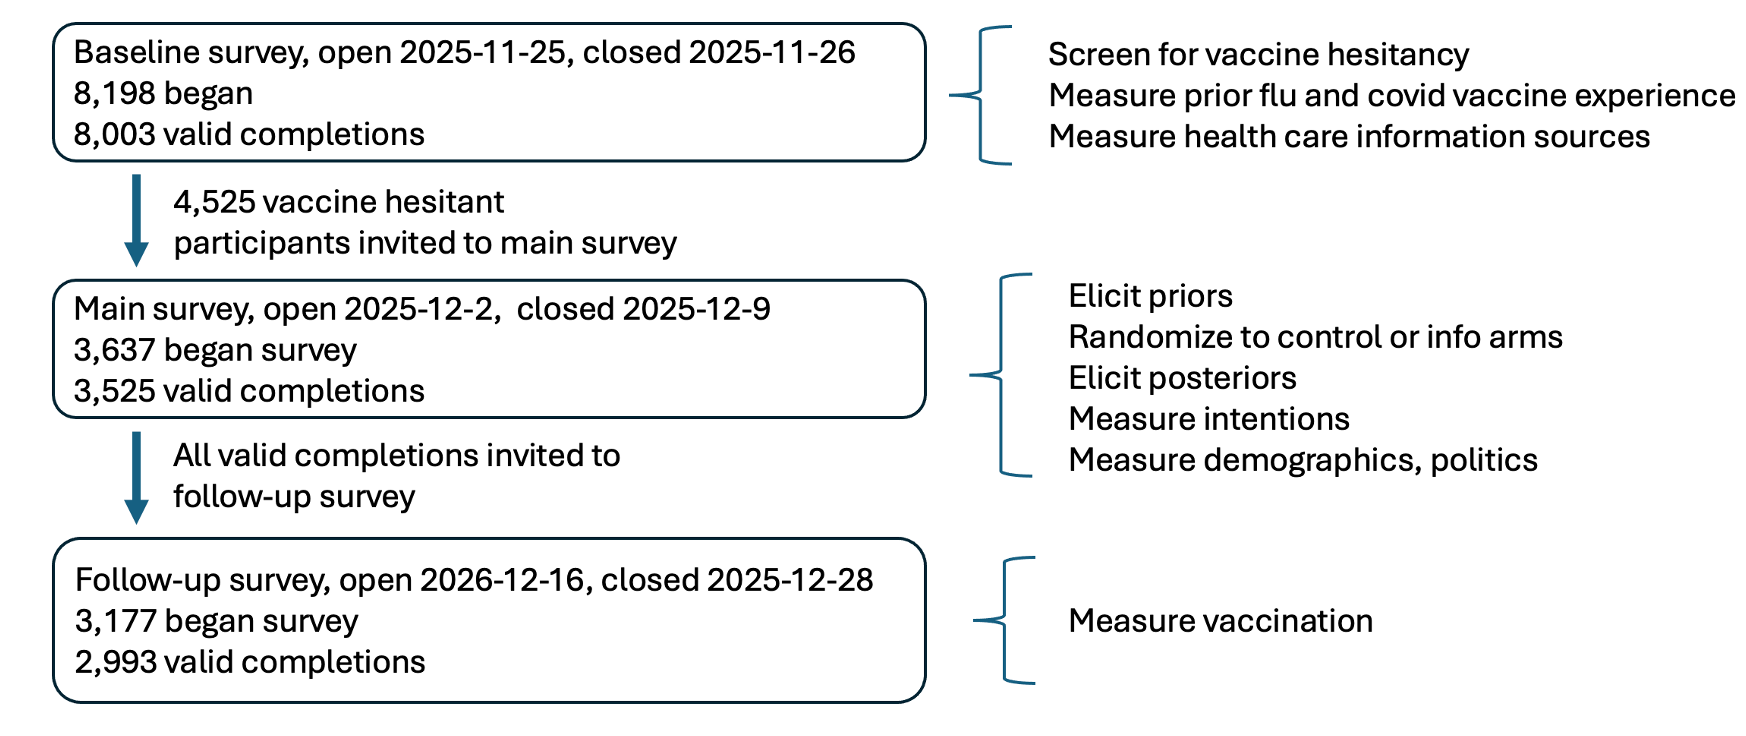
\includegraphics[width=\linewidth]{../notes/study_flow.png}
\fignote{\linewidth}{Notes: Figure reports the timing and sample sizes
of each survey wave. }
\end{figure}

\clearpage

\begin{figure}
\caption{Belief updating and intent effects by perceived trial quality}
\label{fig:hte_quality}
\includegraphics[width=\linewidth]{../output/figures/hte_pca.png}
\fignote{\linewidth}{Notes: Figure reports the effect of industry arm, academic arm, 
or representative arm on beliefs (top row) or vaccine intentions (bottom row), by
perceived trial quality. 
Effect sizes are based on Equation \ref{eq:hte_quality}, which assumes treatment effects 
are linear in quality. See text for details. Shaded area is 95\% confidence interval. }
\end{figure}


\clearpage
\appendix
\setcounter{table}{0}
\renewcommand{\thetable}{A.\arabic{table}}

%==============================================================================
% Appendix Tables
%==============================================================================

%------------------------------------------------------------------------------
% Table A.1: Sample counts by treatment arm and outcome
%------------------------------------------------------------------------------
\begin{table}[htbp]
\centering
\caption{Sample counts by treatment arm and outcome}
\label{tab:counts}
\begin{tabular}{l ccccc}
\toprule
 & (1) & (2) & (3) & (4) & (5) \\
 & Personal SE belief & Trial belief & Vacc.\ intent & Link click & Vaccinated \\ \midrule
Control &   882 &   882 &   879 &   882 &   743 \\
Industry &   878 &   878 &   876 &   878 &   755 \\
Academic &   880 &   880 &   876 &   880 &   746 \\
Representative &   885 &   885 &   885 &   885 &   749 \\
All & 3,525 & 3,525 & 3,516 & 3,525 & 2,993 \\
\bottomrule
\end{tabular}
\tabnote{\linewidth}{Notes: Each cell reports the number of main-survey
respondents in the indicated treatment arm with non-missing values for the
indicated outcome. Column 3 (vaccination intention) has slightly fewer
observations due to missing responses to the intention question. Column 5
(vaccinated) reports follow-up survey respondents, reflecting attrition
between the main and follow-up surveys. See Table~\ref{tab:treat_effects}
for outcome definitions.}
\end{table}

\clearpage

%------------------------------------------------------------------------------
% Table A.2: Treatment effects on trust and relevance perceptions
%------------------------------------------------------------------------------
\begin{table}[htbp]
\centering
\caption{Treatment effects on trust and relevance perceptions}
\label{tab:trust_relevance}
\begin{tabular}{l cccc}
\toprule
 & (1) & (2) & (3) & (4) \\
 & Trust in trial & Relevance of trial & Trust in acad.\ study & Relevance of acad.\ study \\ \midrule
Industry            &      -0.449&       0.033&            &            \\
                    &     (0.102)&     (0.134)&            &            \\
Academic            &      -0.307&      -0.114&            &            \\
                    &     (0.100)&     (0.133)&            &            \\
Representative      &      -0.416&      -0.248&      -0.136&      -0.252\\
                    &     (0.101)&     (0.135)&     (0.103)&     (0.137)\\
Control/Academic mean&       5.751&       5.111&       5.957&       5.046\\
N                   &       3,520&       3,520&       1,762&       1,762\\
 \\
\bottomrule
\end{tabular}
\tabnote{\linewidth}{Notes: Each column is a separate OLS regression of the
indicated outcome on treatment arm indicators, with pre-specified controls
included but not shown. Robust standard errors in parentheses. Outcomes are
measured on a 0--10 scale. Columns 1--2 use all four arms with Control as the
omitted category. Columns 3--4 are restricted to Academic and Representative
arm respondents, as the academic study trust and relevance questions were only
asked of those arms; Academic is the omitted category so only the
Representative arm coefficient is reported. The base mean for columns 3--4 is
the Academic arm mean.}
\end{table}

\clearpage

%------------------------------------------------------------------------------
% Table A.3: Treatment effects on personal SE belief by prior flu vaccine experience
%------------------------------------------------------------------------------
\begin{table}[htbp]
\centering
\caption{Treatment effects on personal side-effect belief by prior flu vaccine experience}
\label{tab:hte_flu_vacc}
\begin{tabular}{l cccc}
\toprule
 & (1) & (2) & (3) & (4) \\
 & No vaccine & No reaction & Mild reaction & Severe reaction \\ \midrule
\input{../output/tables/het_flu_vacc_experience.tex} \\
\bottomrule
\end{tabular}
\tabnote{\linewidth}{Notes: Each column is a separate OLS regression of
personal side-effect belief ($\tilde{\Delta}$) on treatment arm indicators
(Industry, Academic, Representative), with Control as the omitted category.
The sample is split by prior flu vaccine experience: never vaccinated (column
1), vaccinated with no reaction (column 2), vaccinated with a mild reaction
(column 3), and vaccinated with a severe reaction (column 4). Pre-specified
controls are included but not shown. Robust standard errors in parentheses.
The bottom row indicates the subgroup for each column.}
\end{table}

\clearpage

%------------------------------------------------------------------------------
% Table A.4: Heterogeneous treatment effects by predicted trust/relevance index
%------------------------------------------------------------------------------
\begin{table}[htbp]
\centering
\caption{Heterogeneous treatment effects by predicted trust and relevance}
\label{tab:hte_pca}
\begin{tabular}{l cc}
\toprule
 & (1) & (2) \\
 & Personal SE belief & Vacc.\ intention \\ \midrule
Treatment: industry arm&      -3.300&      -0.001\\
                    &     (1.024)&     (0.012)\\
Treatment: academic arm&      -2.901&       0.031\\
                    &     (1.010)&     (0.012)\\
Treatment: personal arm&       0.369&       0.025\\
                    &     (1.021)&     (0.012)\\
Fitted values, penalized&      -1.311&       0.038\\
                    &     (1.961)&     (0.022)\\
Fitted values, penalized $\times$ Treatment: industry arm&      -2.985&       0.041\\
                    &     (1.779)&     (0.019)\\
Fitted values, penalized $\times$ Treatment: academic arm&      -1.982&       0.051\\
                    &     (1.820)&     (0.019)\\
Fitted values, penalized $\times$ Treatment: personal arm&      -2.439&       0.063\\
                    &     (1.885)&     (0.019)\\
Control mean        &      15.427&       0.069\\
N                   &       3,525&       3,516\\
 \\
\bottomrule
\end{tabular}
\tabnote{\linewidth}{Notes: Each column is a separate OLS regression of the
indicated outcome on treatment arm indicators (Industry, Academic,
Representative), a predicted trust/relevance index (\texttt{pca1\_hat}), and
interactions of each arm indicator with the index. \texttt{pca1\_hat} is the
first principal component of post-treatment trust in the clinical trial and
perceived relevance of the trial, predicted from pre-experiment covariates
using lasso selected in the control group. Rows labeled ``Fitted values,
penalized'' report the coefficient on \texttt{pca1\_hat}; interaction rows
report the coefficient on the arm-by-index interaction. Pre-specified controls
are included but not shown. Robust standard errors in parentheses. See
Table~\ref{tab:treat_effects} for outcome definitions.}
\end{table}


\clearpage
\setcounter{figure}{0}
\renewcommand{\thefigure}{A.\arabic{figure}}

%==============================================================================
% Appendix Figures
%==============================================================================

%------------------------------------------------------------------------------
% Figure A.1: All four experiment conditions
%------------------------------------------------------------------------------
\begin{figure}[htbp]
\caption{Experiment conditions}
\centering
\setlength{\fboxsep}{3pt}
\setlength{\fboxrule}{0.6pt}
\begin{tabular}{cc}
\fbox{
\includegraphics[width=0.46\textwidth]{../slides/control.png}} &
\fbox{
\includegraphics[width=0.46\textwidth]{../slides/industry.png}} \\[4pt]
(a) Control & (b) Industry \\[14pt]
\fbox{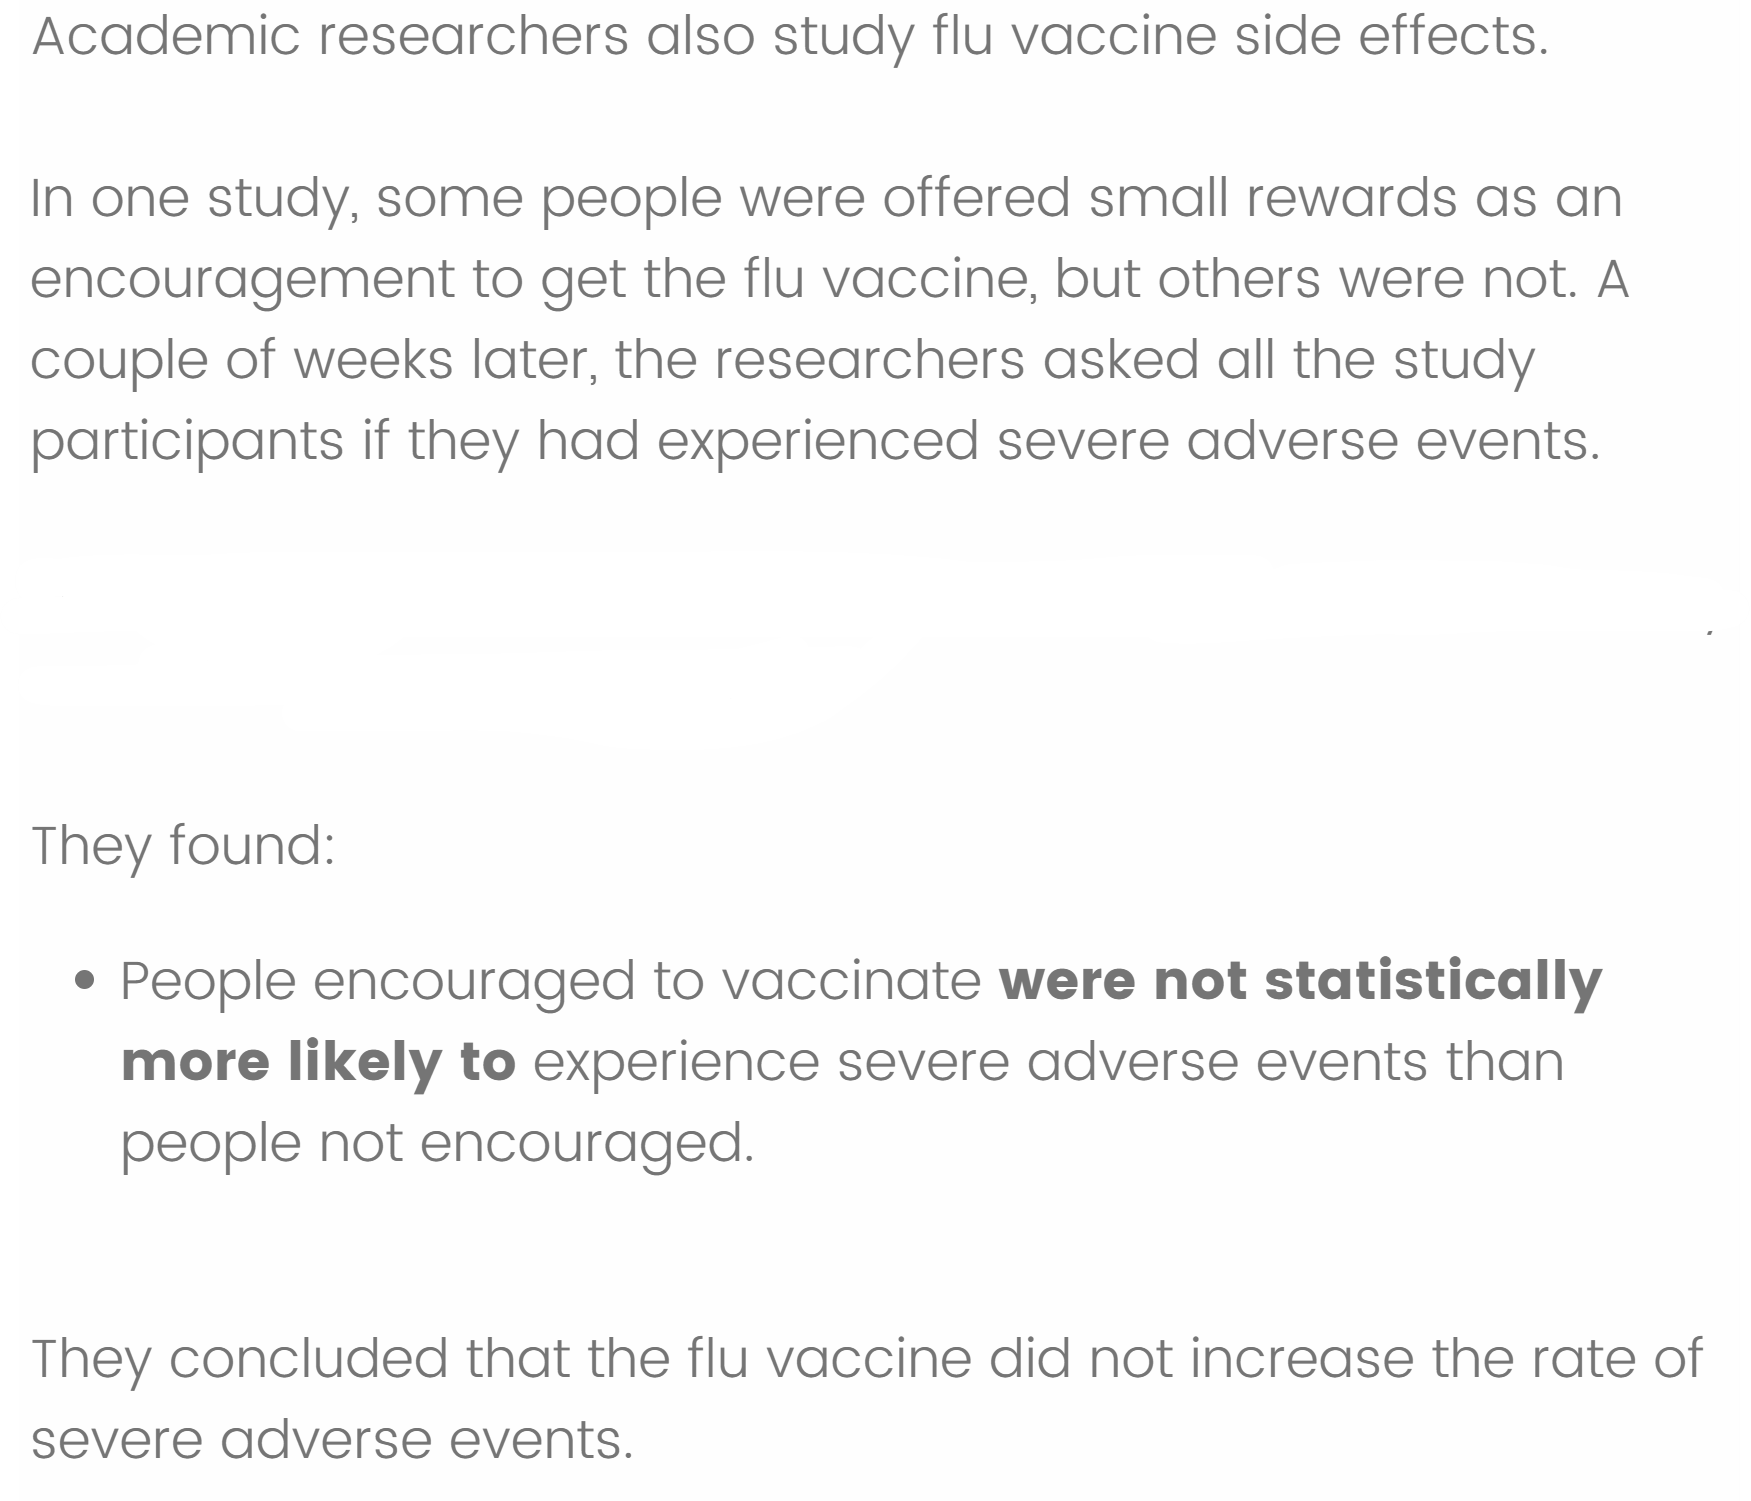
\includegraphics[width=0.46\textwidth]{../slides/academic.png}} &
\fbox{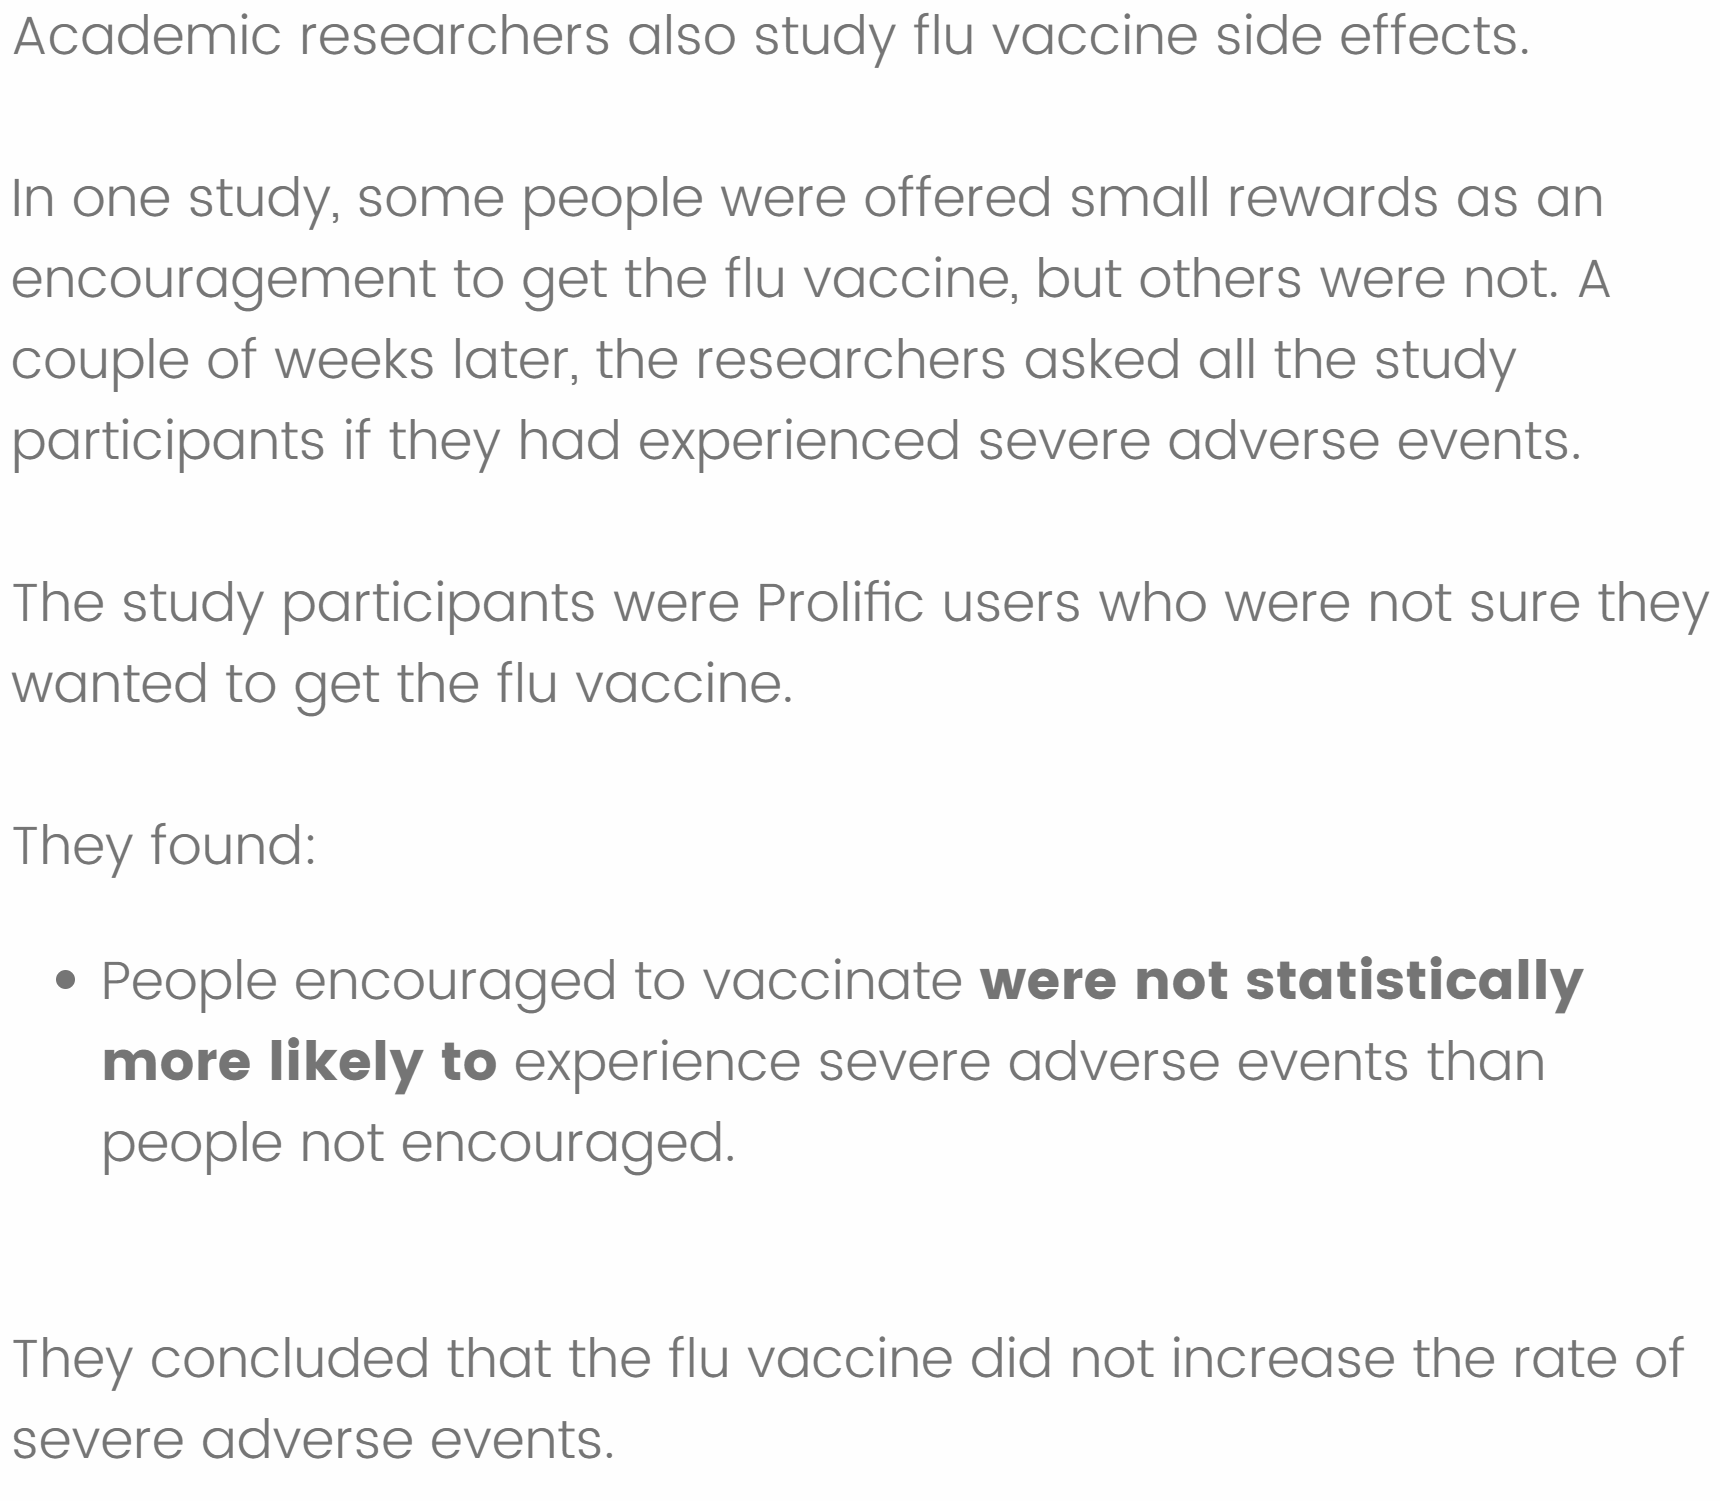
\includegraphics[width=0.46\textwidth]{../slides/personal.png}} \\[4pt]
(c) Academic (additional info beyond control) & (d) Representative  (additional info) 
beyond controls\\
\end{tabular}
\label{fig:interventions}
\fignote{\linewidth}{Screenshots of the information screens for all four
treatment arms. Participants in the academic and representative arms saw 
the control arm information as well as the information about the academic study.}
\end{figure}



\begin{figure}
\caption{Trust in government and following doctor's advice by vaccine hesitancy}
\label{fig:trust_by_hes}
\centering 
\includegraphics[height=0.8\textheight]{../output/figures/trust_by_hes.png}
\fignote{\linewidth}{Notes: Top panel reports s the fraction of vaccine hesitant
and non-hesitant participants who report using the indicated source "sometimes"
or "often" for health care information. Bottom panel reports the fraction 
who view the source as "reliable" (as opposed to "somewhat reliable" or "not reliable"),
conditional on using that source. }
\end{figure}

\end{document}
